\documentclass[problems]{esg8022pset} 
  \usepackage{amsmath}
  \usepackage{amssymb}
  \usepackage{enumerate}
  \usepackage{graphicx}
  \usepackage{hyperref}
  \usepackage{mathtools}
  \usepackage[per-mode=symbol,exponent-product=\cdot]{siunitx} %If this line is giving you trouble, try replacing per-mode with per
  \providecommand{\uvec}[1]{{\hat{\bf{#1}}}}
  \usepackage{pgf,tikz}
  \usetikzlibrary{arrows}
  \usepackage{wasysym}
  \usepackage{subfig}
  \usepackage{wrapfig}
  \makeatletter
  \newcommand{\interitemtext}[1]{%
    \begin{list}{}
     {\itemindent=0mm\labelsep=0mm
     \labelwidth=0mm\leftmargin=0mm
     \addtolength{\leftmargin}{-\@totalleftmargin}}
      \item #1
    \end{list}
  }
  \makeatother
  \renewcommand{\d}{\,d}
  \providecommand{\norm}[1]{\lVert#1\rVert}

  \AtBeginDocument{%
    % Appologies to any future editor on the inconsistencies in TeX code and the unnecessary braces.  I'm aggregating previously typeset problems, and didn't think it worth my time to improve the quality of TeX code in ways that won't make any difference to the typeset material. -Jason Gross (jgross@mit.edu)
  }%
\classname{Physics 8.022} \semester{Spring 2011} 
\problemsetnumber{6}
\date{\today }
\duedate{Sunday, March 13 at 10 \textsc {pm}}
\readingassignment{}
\problemsettitle{Resistances and Circuits}
\begin{document}
\section{Problem \thesection: Purcell 4.4: Resistance of Atlantic Ocean}
  The first telegraphic messages crossed the Atlantic Ocean in 1858, by a cable 3000 km long laid between Newfoundland and Ireland. The conductor in this cable consisted of seven copper wires, each of diameter 0.73 mm, bundled together and surrounded by an insulating sheath.
  \begin{enumerate}[(a)]
    \item Calculate the resistance of the conductor. Use \SI{3e-8}{\ohm\meter} for the resistivity of copper, which was of somewhat dubious purity.
    \item A return path for the current was provided by the ocean itself. Given that the resistivity of seawater is about \SI{0.25}{\ohm\meter}, see if you can show that the resistance of the ocean return would have been much smaller than that of the cable.
  \end{enumerate}
\section{Problem \thesection: Sea Water}
  \begin{wrapfigure}{r}{0.25\textwidth}
    \begin{center}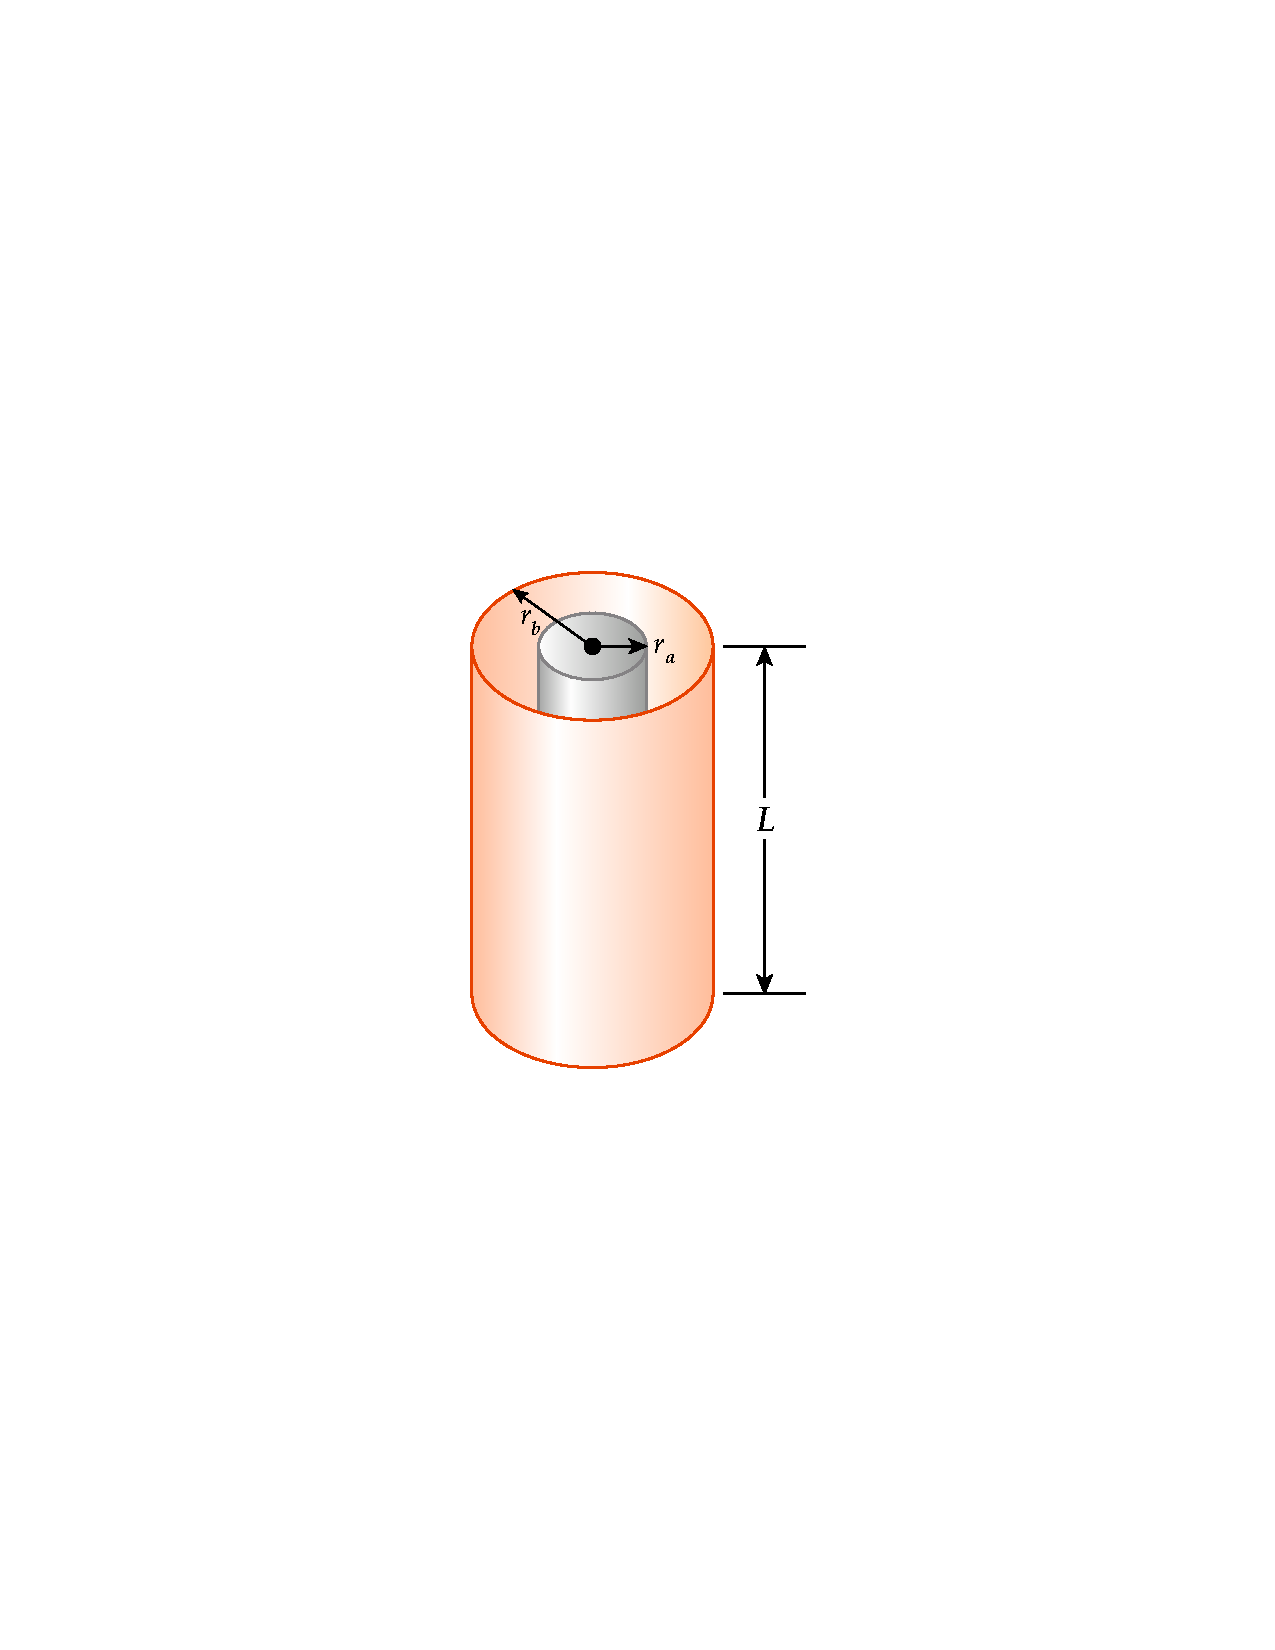
\includegraphics[width=0.20\textwidth]{ps06_02_01.pdf}\end{center}
  \end{wrapfigure}
  An oceanographer is studying how the ion concentration in sea water depends on depth. She does this by lowering into the water (until completely submerged) a pair of concentric metallic cylinders (see figure) at the end of a cable and taking data to determine the resistance between these electrodes as a function of depth. The water between the two cylinders forms a cylindrical shell of inner radius $r_a$, outer radius $r_b$, and length $L$ much larger than $r_b$. The scientist applies a potential difference $\Delta V$ between the inner and outer surfaces, producing an outward radial current $I$. Let $\rho$ represent the resistivity of the water.
  \begin{enumerate}[(a)]
    \item Find the resistance of the water between the cylinders in terms of $L$, $\rho$, $r_a$, and $r_b$.
    \item Express the resistivity of the water in terms of the measured quantities $L$, $r_a$, $r_b$, $\Delta V$, and $I$.
  \end{enumerate}
\section{Problem \thesection: Non-uniform Conductivity}
  A cylindrical glass rod is heated with a torch until it conducts enough current to cause a light bulb to glow. The rod has a length $L = 2$ cm, a diameter $d = 0.5$ cm, and its ends, plated with material of infinite conductivity, are connected to the rest of the circuit. When red hot, the rod's conductivity varies with position $x$ measured from the center of the rod as $\sigma(x) = \sigma_0 L^4 / x^4$, with $\sigma_0 = 4 \cdot 10^{-2} (\Omega\cdot{\rm m})^{-1}$.
  \begin{enumerate}[(a)]
    \item What is the resistance of the glass rod? Express your answer both symbolically and as a value in ohms.
    \item When a voltage $\Delta V$ is applied between the two ends, what is the current density $\vec J(x)$ and what is the steady-state electric field $\vec E(x)$?
    \item In steady-state, what is the volume charge density $\rho(x)$ found within the rod? (Note that you are not asked for the surface charge $\sigma$ that will accumulate on the surfaces.)
  \end{enumerate}
\section{Problem \thesection: Battery Lifetime}
  A standard D cell can supply 10 mA at 1.5 V for about 300 hours. An alkaline D cell can do about the same. Assume that the chemistry of the batteries will produce the same amount of energy and will maintain the emf $\epsilon = 1.5$ V regardless of the current drawn from the battery. However the internal resistance of a standard D cell is about 1 $\Omega$ and the internal resistance of an alkaline D cell is about 0.1 $\Omega$, so the amount of energy dissipated internally is different. Suppose that you have a multi-speed winch that is 50\% efficient, and that you are trying to lift a mass of 60 kg. The winch acts as load with a variable resistance $R_L$ at different speeds.
  \begin{enumerate}[(a)]
    \item Suppose the winch is set to super-slow speed. Then the load resistance is much greater than the internal resistance and you can assume that there is no loss of energy to internal resistance. How high can each battery lift the mass before the battery uses all of its energy?
    \item For each battery, what should the resistance of the winch be set at in order to have the battery lift the mass at the fastest rate?
    \item What is the fastest rate in m/sec that each battery can lift the mass?
    \item At this fastest lift rate, what is the maximum height that you can lift the mass before the battery dies?
    \item How long does it take to reach this height?
  \end{enumerate}
\section{Problem \thesection: Purcell 4.16}
  In the circuit below, if $R_0$ is given, what value must $R_1$ have in order
  that the input resistance between the terminals shall be equal to $R_0$?

  \begin{center}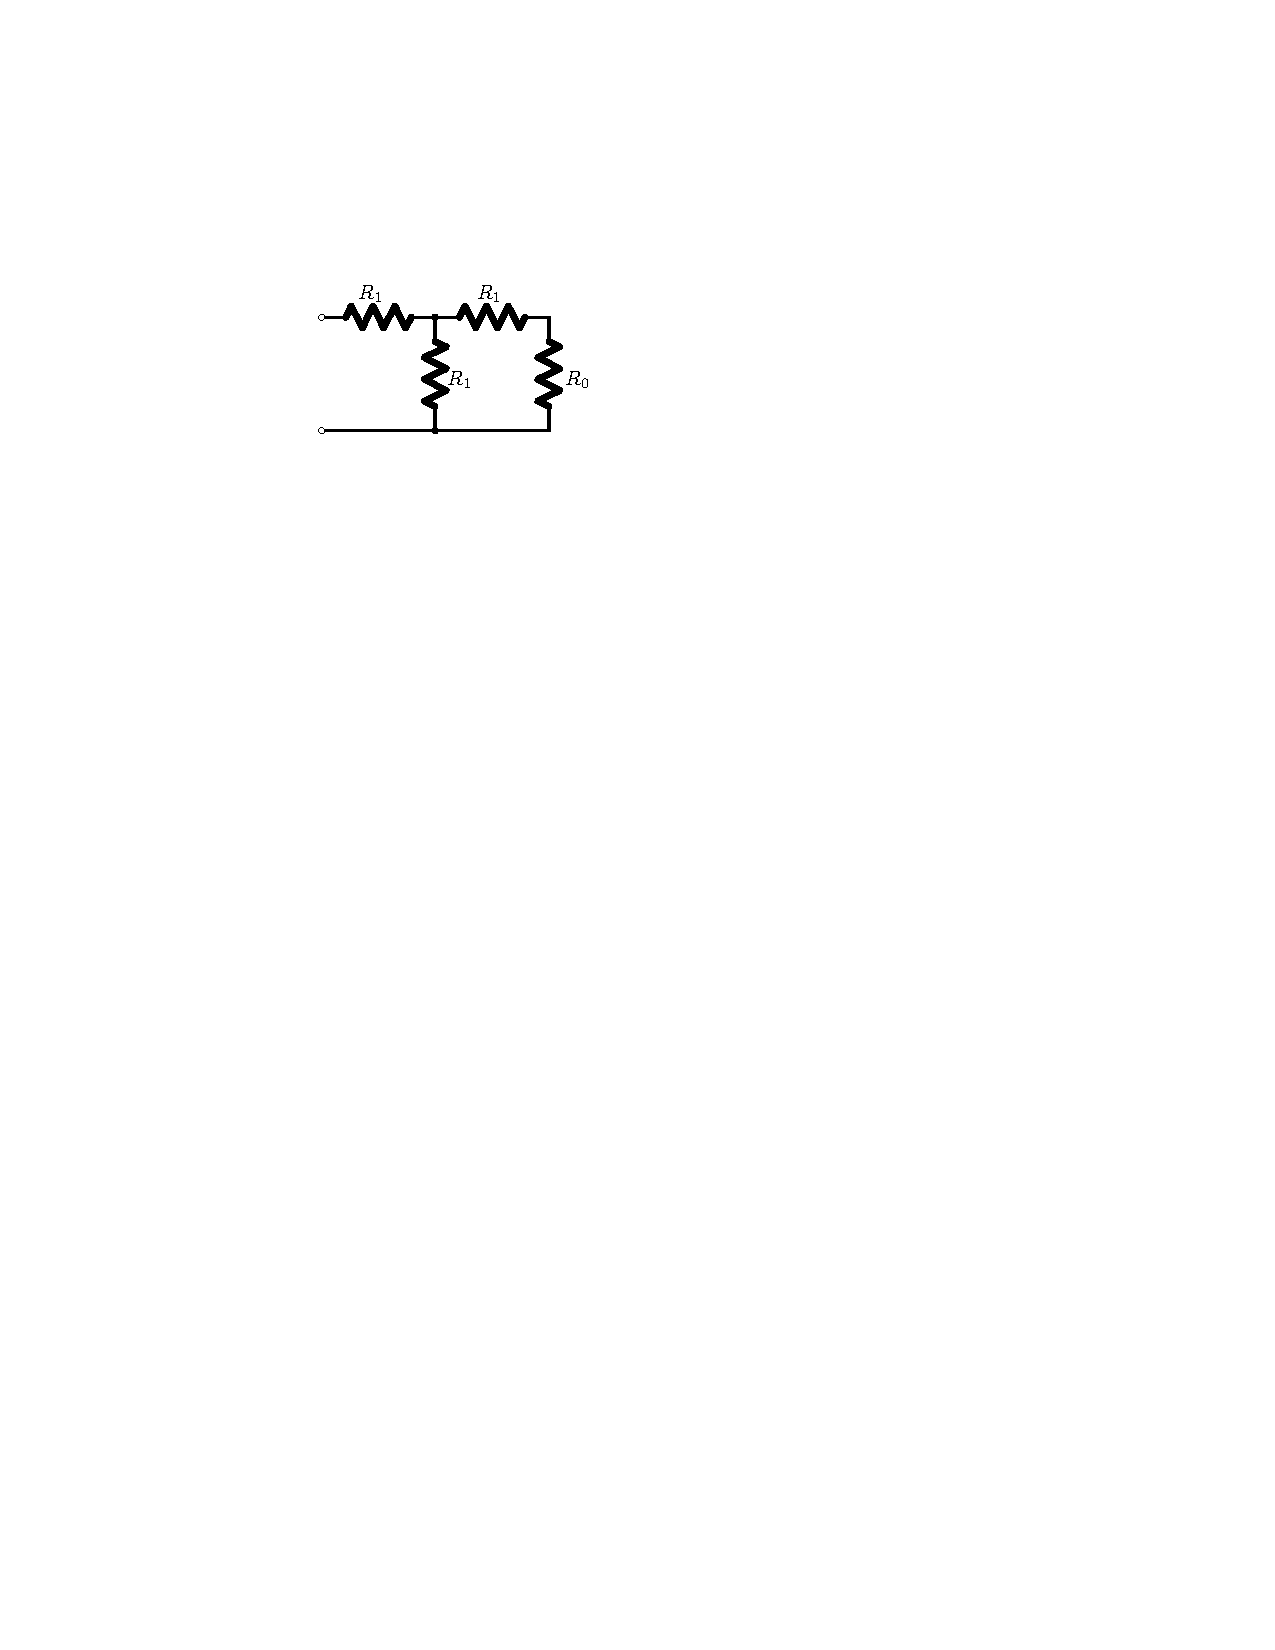
\includegraphics[width=0.4\textwidth]{ps06_05_01.pdf}\end{center}
\section{Problem \thesection: Purcell 4.19: Design an ohmmeter}
  You own a micro-ammeter that reads \SI{50}{\micro\ampere} at full scale deflection, and the coil in the meter movement has a resistance of 20 $\Omega$. By adding two resistors, $R_1$ and $R_2$, and a 1.5 V battery you can convert this into an ohmmeter. When the two outgoing leads of this ohmmeter are connected together, the meter should register 0 ohms by giving full-scale deflection. When the leads are connected across an unknown resistance $R_u$, the deflection will indicate the resistance value if the scale is appropriately marked. In particular, we want half-scale deflection to indicate 15 $\Omega$. What values of $R_1$ and $R_2$, are required, how should the connections be made, and where on the ohm scale will the marks be (with reference to the old micro-ammeter calibration) for 5 $\Omega$ and 50 $\Omega$? Are there several different combinations that can solve this problem?
\section{Problem \thesection: Composite Conducting Medium}
  \begin{wrapfigure}{r}{0.2\textwidth}\vspace{-5\intextsep}
    \begin{center}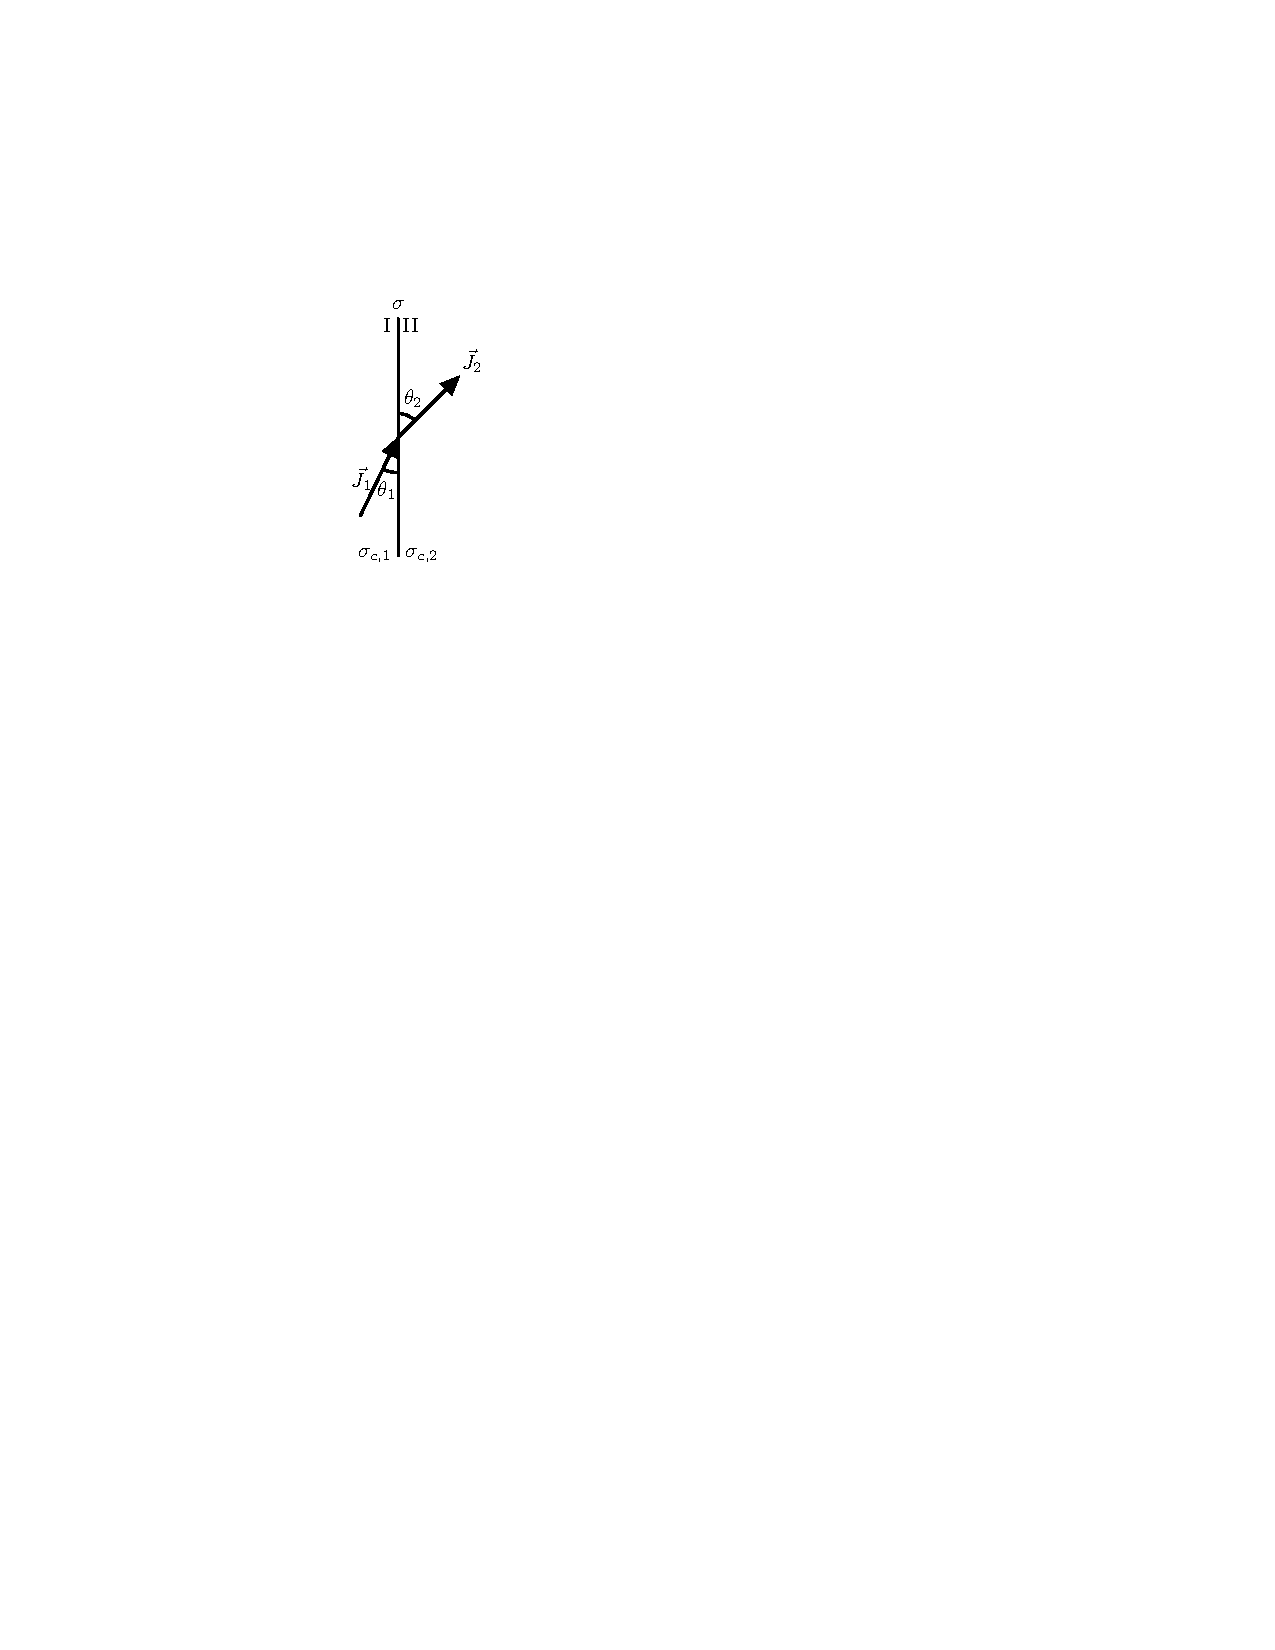
\includegraphics[width=0.15\textwidth]{ps06_07_01}\end{center}
  \end{wrapfigure}
  An infinite conducting medium has two regions with conductivity $\sigma_{c,1}$ and $\sigma_{c,2}$, separated by a plane interface. In
  region 1 a uniform current density $\vec J_1$ flows up to the interface, making at an angle $\theta_1$ with the interface. $\vec J_2$ flows away from the interface and makes an angle $\theta_2$ with the interface. Assume that the charge density $\sigma$ is not changing in time.
  \begin{enumerate}[(a)]
    \item Find the direction and magnitude of the current density $\vec J_2$ in region 2.
    \item Find the surface charge density $\sigma$ on the interface.
  \end{enumerate}
\section{Problem \thesection: Multiple Loop Circuits}
  Consider the following circuit consisting of a voltage source $V_0$ , three resistors with resistances $R_1$, $R_2$, and $R_3$, and a capacitor with capacitance $C$ connected together as shown in the Figure below.
  \begin{center}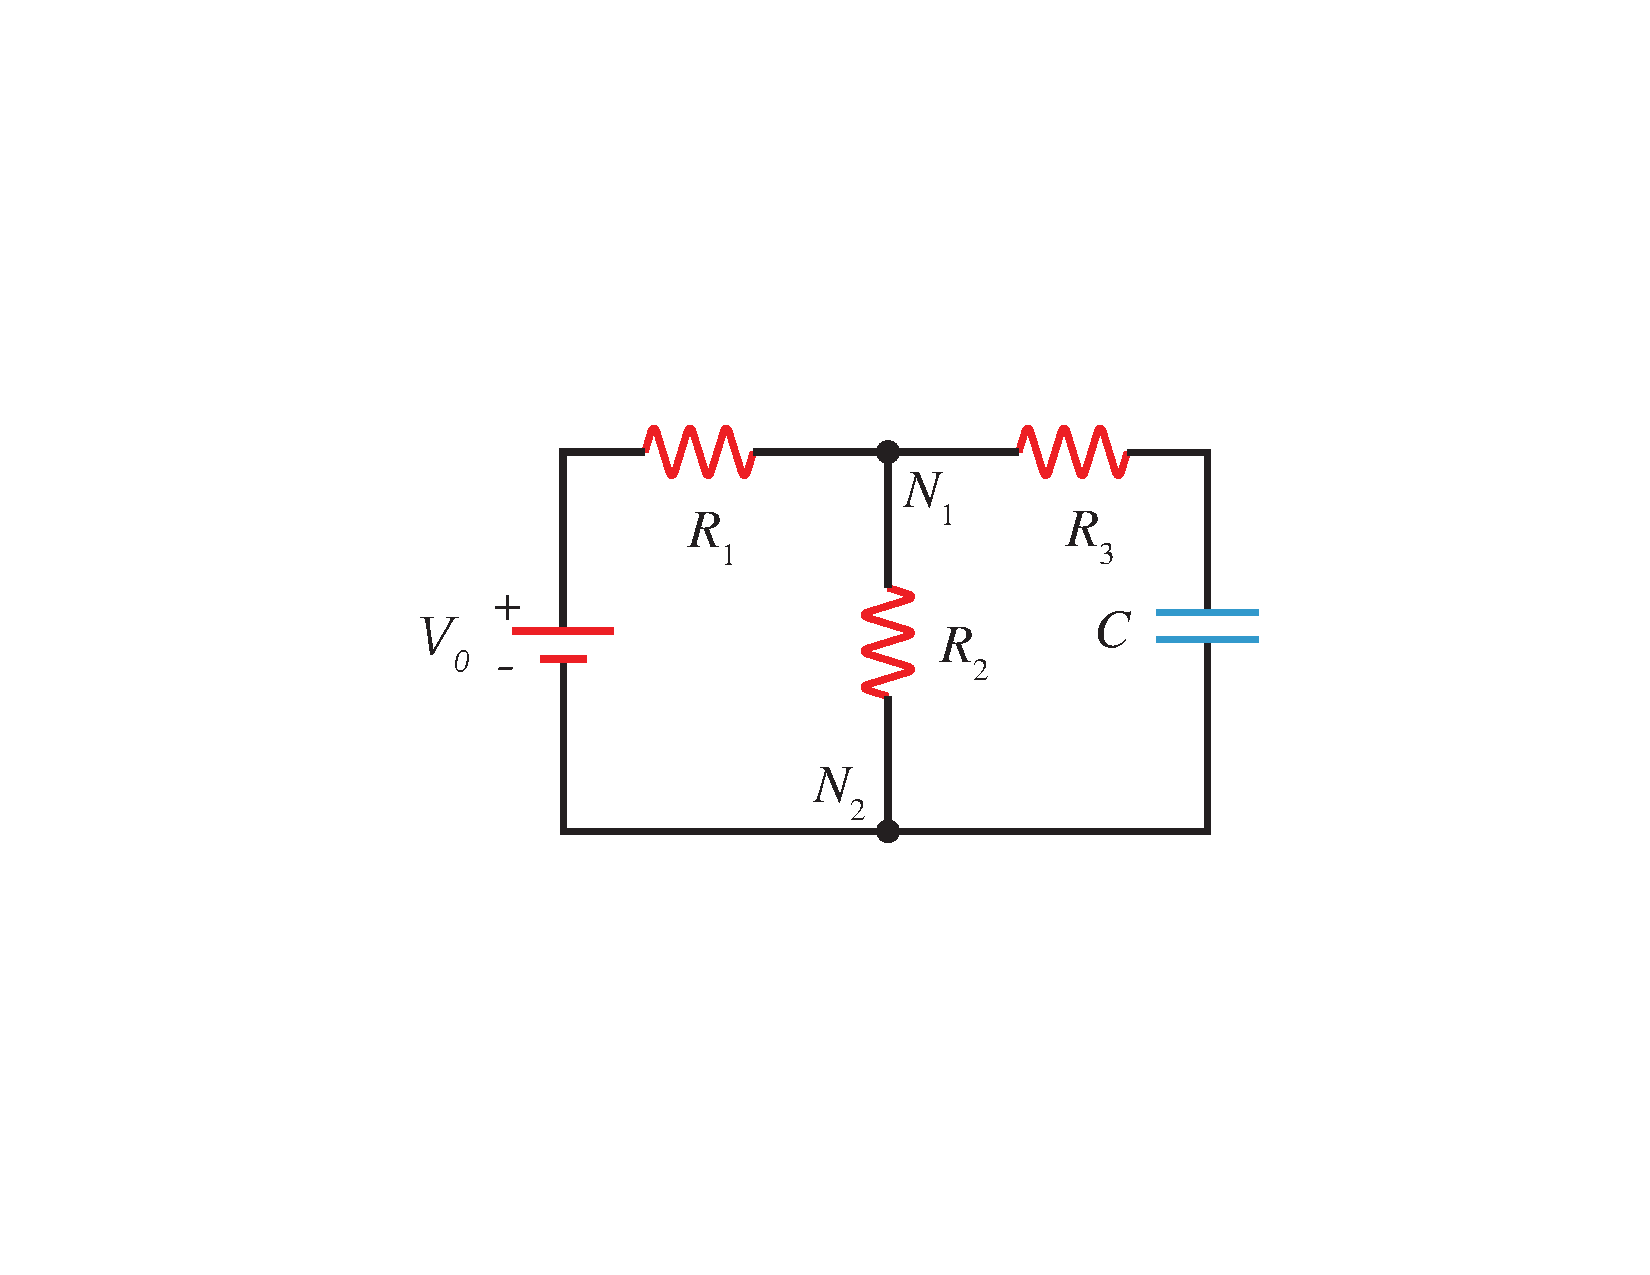
\includegraphics[width=0.4\textwidth]{ps06_08_01}\end{center}
  \begin{enumerate}[(a)]
    \item Find a differential equation for the charge on the capacitor and try to solve it.
    \item What is the time constant for this circuit?
    \interitemtext{\textbf{Try to answer the following questions conceptually then check your answer against your solutions.}}
    \item At $t = 0$, what is the voltage difference across the capacitor?
    \item What is the current that flows in the branch containing the voltage source at $t = 0$.
    \item When a long time has passed after the switch was closed, what is the current that flows in the branch of the circuit that included the capacitor?
    \item When a long time has passed after the switch was closed (based on your result form part e), find the current that flows from the voltage source?
  \end{enumerate}
\section{Problem \thesection: Infinite Lattice of Resistors}
  Suppose you have an infinite lattice of resistors, all of the same resistance $R$, as illustrated in the figure. Suppose you apply a potential difference between two adjacent nodes C and D which causes a current of $I = 1$ A to flow into C and a current of $I = 1$ A to flow out of D.
  \begin{enumerate}[(a)]
   \item How much current flows through the resistor connecting C to D?
   \item What is the total resistance $R_{CD}$ of the lattice between the two points?
  \end{enumerate}
  \begin{center}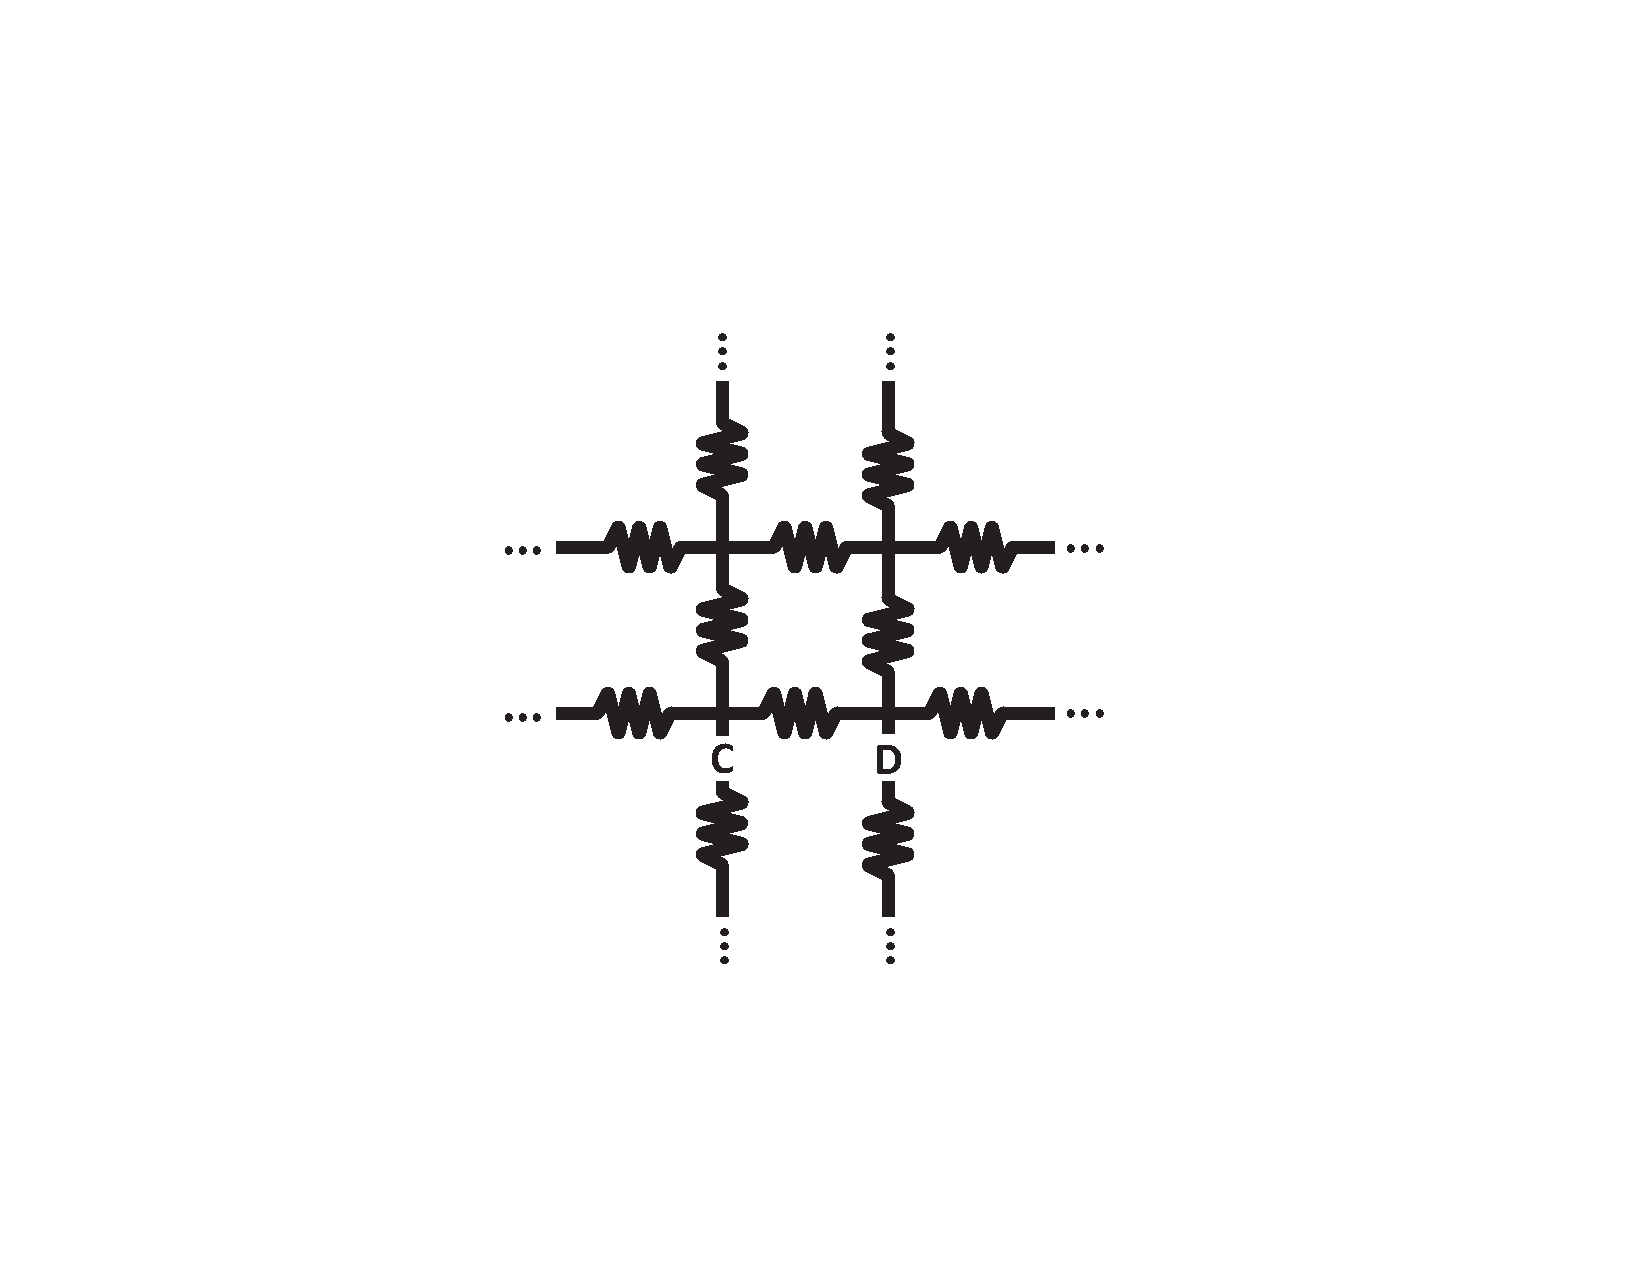
\includegraphics[width=0.33\textwidth]{ps06_09_01}\end{center}
\end{document}
